% DNS defined in the intro!
\subsection{Incompressible DNS Application}
\label{sec:dns_full}

% Why DNS code needs to be improved
Direct numerical simulation (DNS) plays an important role in
understanding turbulent flows because DNS provides high fidelity data
that is difficult to obtain experimentally. After Kim {\it et al.}
first used the DNS for wall-bounded turbulence flow in 1987
\cite{Kim:1987ub}, DNS has been used extensively to understand the
turbulence phenomenon and to help develop models of turbulence.
Turbulence is characterized by a non-dimensional parameter known
as the Reynolds Number ($Re$).  The vast majority of fluid flows
in industry and nature occur at large $Re$.
However, as $Re$ increases, time and length scales become smaller.
Thus, DNS at high $Re$ naturally requires a fine meshes and time-steps
to obtain meaningful data from flows of interest.
Therefore, the use of state-of-art HPC systems is mandated
 to study turbulent flows of interest. To date, the highest
$Re$ of the wall-bounded turbulence DNS was at $\approx 250,000$,
which required 242 billion degrees of freedom to
resolve\cite{Lee:2015er}. However, $Re$ = 250,000 remains substantially
lower than the $Re$  for many practical engineering applications.
To enable DNS at these higher $Re$, at least exascale
capable HPC systems are required. These systems will require
not only substantial hardware advanced, but also modifications
to the underlying DNS codes.

% Detail of simulation
In this section, we will show you the results of testing PoongBack on
KNL nodes in Stampede, which is a channel flow DNS code optimized for
the modern HPC systems. PoongBack,
named after the ancient Korean god of winds,
simulates a channel flow: the flow between two infinite
parallel plates. The simulation code
has already been scaled to several top-10 HPC systems, and has
shown excellent performance during its use by several research
groups\cite{Lee:2013kv}. In particular, it was used for
generating the data for the NSF supported virtual flow laboratory in the
Johns Hopkins Turbulence Data Base\cite{Graham:2015ha}.
The code uses the Fourier-Galerkin spectral method in the streamwise and spanwise directions
and a high-order basis spline method in the wall-normal direction.
For time integration PoongBack uses a low-storage
third-order Runge-Kutta method\cite{Spalart:1991wu}.
The simulation domain is partitioned by
a two-dimensional decomposition, a.k.a. pencil-decomposition. PoongBack
contains three major kernels; (1) solving the Navier-Stokes equations in
a complex domain (2) one-dimensional fast Fourier transforms (3)
data transpose in two dimension. The combination of (2) and (3) provides 3D
FFTs and there are many existing libraries for it. We developed a customized 3D
FFT library because of the needs for zero-padding for 3/2
dealiasing. Additionally, PoongBack uses a customized I/O library for the HDF-5
format, ESIO~\cite{Lee:2014ta}, which has been shown to be performant to
large core counts, but the I/O performance is beyond the scope of the current work.
See \cite{Lee:2013kv,Lee:2014ta} for more details about PoongBack.

For this study the grid size used was $1024\times128\times512$, which is
comparable to the $Re_\tau = 180$ simulation from
Kim\cite{Kim:1987ub}. For every benchmark cases, MCDRAM is
used as a cache memory between processors and DRAM. The simulation code
was compiled with the flag ``{\tt -xMIC-AVX512}.'' Also, the FFTW-3.3.5
library is installed with the options ``{\tt --enable-avx512}'' and
``{\tt --enable-mpi}.''~\cite{Frigo:2005tu}. We used double-precision
operations for all the kernels and elapsed times were measured by ``{\tt
mpi\_wtime()}'' with ``{\tt mpi\_barrier()}.''

\begin{figure}
 \begin{center}
   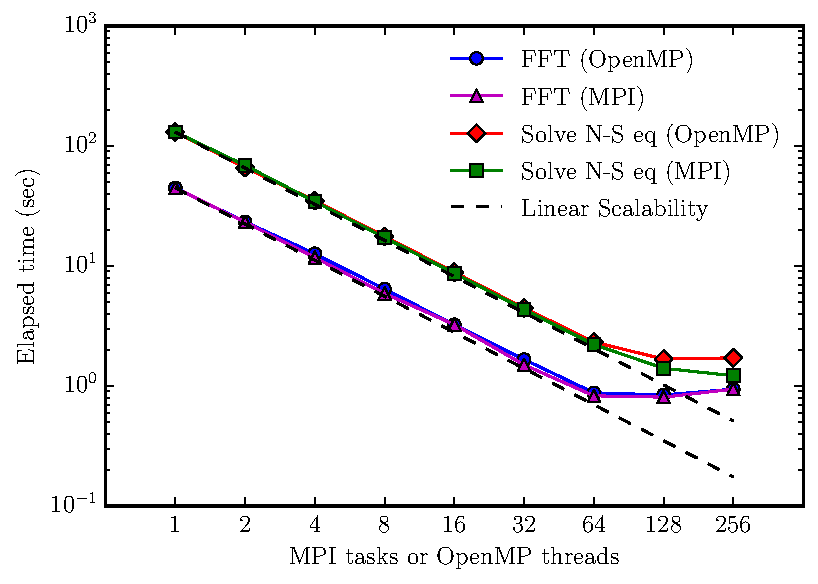
\includegraphics[width=0.45\textwidth]{DNS_FFT_Wave}
   \caption{Strong scaling result depicting 1D FFTs and the solution of the
  N-S equations in wavespace for a single timestep.}
   \label{fig:DNS_strong_scale_fft_wave}
 \end{center}
\end{figure}

% 1D FFT and wavespace performance
Figure~\ref{fig:DNS_strong_scale_fft_wave} shows the strong scaling performance
of the kernels involving floating point operations; 1D FFTs and solving the
Navier-Stokes equations. Four different FFTs are performed; real-to-complex
(R2C), complex-to-real (C2R), forward complex-to-complex (fC2C) and backward
complex-to-complex (bC2C). Before or after each FFT, 1d contiguous data lines
are padded or truncated with zeros.  Also, nonlinear products such as $A\times
B \rightarrow C$ were performed between C2R and R2C transforms. The elapsed
time for 1D FFTs, zero padding/truncation and nonlinear product are shown in
Figure~\ref{fig:DNS_strong_scale_fft_wave} in blue and magenta. In both cases
using either MPI-only and OpenMP-only the performance is almost linear up to 64
processors. When two hardware threads were used per core (hyperthreading), the
performance did not increase. Furthermore, the performance decreases when four
hardware threads were used in both MPI and OpenMP cases. The performance was
best with 64 processors and showed 270 GFlops, or approximately 9\% of peak
performance. This means that the performance of 1D FFTs on KNL nodes are memory
bandwidth limited.

There are numerous floating point operations involved in the compute
kernels for solving the Navier-Stokes equations.
Particularly critical numerical operations include solving the linear system
$A \textbf{x} = \textbf{b}$, along with
matrix-vector multiplications. The matrix $A$ is a banded matrix with
additional non-zero elements in several first and last rows. Also, the
elements of $A$ are real while the elements of $\textbf{x}$ and
$\textbf{b}$ are complex. To take advantage of these properties, we have
implemented a customized linear algebra solver. As the Navier-Stokes
equation is solved in a complex number domain, after the 1D FFTs in two
directions, the 3D PDE is decoupled and becomes a series of 1D ODEs, one
for each wavenumber. In this way, the
Navier-Stokes equations are solved concurrently at each wavenumber without
interaction between wavenumbers. As a result, this portion of the kernel
is parallelized and requires no communication. The performance of
the kernel for solving the Navier-Stokes equations is shown in
Figure~\ref{fig:DNS_strong_scale_fft_wave} in green and red. Similar to
the FFTs, both MPI-only and OpenMP-only cases were performed and show
almost ideal scalability up to 64 cores.
There were small, but noticeable, performance increases
observed with two hardware threads. Interestingly, the performance of
OpenMP only case decreases while the performance of MPI only case
increases when four hardware threads per core were applied. This could be
due to different memory access patterns between MPI and OpenMP,
or scheduling overhead in OpenMP, which was also observed in Intel's work on
HPCG\cite{Park:2014:ESI:2683593.2683696}.

% Transpose performance
\begin{figure}
 \begin{center}
   \includegraphics[width=0.45\textwidth]{DNS_Transpose}
   \caption{Strong scaling result of data reorder and MPI communication; OpenMP is not used.}
   \label{fig:DNS_strong_scale_transpose}
 \end{center}
\end{figure}

The last kernel of PoongBack is the data transpose in a two
dimensionally partitioned domain. This kernel is to ensure data
alignment for FFTs and linear problems when solving the Navier-Stokes
equations and does not include any floating point operations. However,
more than 50\% of the simulation time occurs during this
operation. The data transpose kernel includes two subsequent parts: 1)
All-to-All type MPI communication in two sub-communicators; and 2)
data reordering to maximize MPI message size and to finalize memory
alignment after MPI communication. As the domain is partitioned in two
dimensions, MPI communication needs to be performed in both
dimensions. This is accomplished using MPI sub-communicators.  The
communication in each direction is logically All-to-All, but other
communication patterns can be faster than ``{\tt mpi\_alltoall}''
depending on the 2D communication topology. We have used MPI-enabled
FFTW (version 3.3 or higher), which dynamically determines the optimal
communication patterns for each sub-communicator. Since MPI-enabled
FFTW only supports a one dimensionally partitioned domain, a.k.a plane
decomposition, we separately use FFTW for 1D FFTs and MPI
communications with ``{\tt fftw\_mpi\_execute\_r2r()}''.\footnote{The
  orignial idea of using FFTW 3.3 library for global transpose is from
  Dr. Rhys Ulerich.} The part of code used for data reordering
performs a tensor transpose: {\tt B(i,j,k,l) $\leftarrow$ A(l,i,k,j)}
or {\tt B(i,j,k) $\leftarrow$ A(j,k,i)}. Unfortunately, cache-line
optimization cannot be achieved for both load and store at the same
time. In this work we preferentially loaded the order of transpose.
The performance of MPI communication and data reordering is shown in
Figure~\ref{fig:DNS_strong_scale_transpose}. Similar to the FFT
scaling and Navier-Stokes scaling in
Figure~\ref{fig:DNS_strong_scale_fft_wave}, data reordering also shows
nearly perfect linear scalability up to 64 cores. Indeed, the
performance continues to increase even with hardware threading.  On
the other hand, profiling the MPI communication shows performance
increases as the number of cores increases even with more than one MPI
tasks for each hardware thread. Admittedly, the scalability is far
from linear. This result is interesting because PoongBack benchmark
results on other HPC systems show that MPI communication takes more
than five times the elapsed time for data
reordering~\cite{Lee:2013kv}. This may imply that the performance
could be increased by fine tuning the data reordering for KNL nodes.

\begin{figure}
 \begin{center}
   \includegraphics[width=0.45\textwidth]{DNS_Parallelism}
   \caption{Comparison of MPI$\times$OpenMP in data transpose}
   \label{fig:DNS_MPI_OpenMP}
 \end{center}
\end{figure}


For data re-ordering, OpenMP can be used in each MPI task. This hybrid MPI+OpenMP parallelism
is tested and results are shown in Figure~\ref{fig:DNS_MPI_OpenMP}.
Each line in Figure~\ref{fig:DNS_MPI_OpenMP} details cases where the product of
the number of MPI tasks and the number of OpenMP threads is
constant. Using more MPI tasks and less OpenMP threads generally shows
better performance. The best performance is achieved when 256 MPI tasks
were used with four hardware threads. This is because using MPI shows
better performance than OpenMP for data reordering. Also, using more MPI
tasks performs better for MPI communication as shown in
Figure~\ref{fig:DNS_strong_scale_transpose}.
%Finally, the size of tensor
%transpose changes with number of MPI tasks.


\begin{figure}
 \begin{center}
   \includegraphics[width=0.45\textwidth]{DNS_full_timestep}
   \caption{Strong scaling results for the total elapsed time for single timestep. The parantheses denote: (MPI tasks $\times$ OpenMP threads).}
%   \caption{Strong scaling results for the total elapsed time for single timestep. The parantheses denote: (MPI tasks $\times$ OpenMP threads). Hybrid parallelism was found to show the best performance, with nearly perfect scalability until approximately 128 concurrencies.}
   \label{fig:DNS_strong_scale_total_elapsed_time}
 \end{center}
\end{figure}

The performance of one full timestep (without I/O) is shown in
Figure~\ref{fig:DNS_strong_scale_total_elapsed_time}. The best
performing set of MPI $\times$ OpenMP concurrency for each number of
processors was chosen. It also shows almost perfect scalability up to 64
processors. The performance continues to increase after using hardware
threads. In most cases, using only MPI tasks shows the best performance,
excepts at 64 processors with 2 hardware threads. However, the
difference between hybrid parallelism and only MPI tasks are minimal at
128 processors. A conclusion from this study is that generally speaking,
using only MPI seems to be the best option for any problem size.
Despite this, we also note that hybrid parallelism could be more
important due to the off-node impact. When the problem size
is bigger than the size of DRAM on a KNL node, one must use multiple KNL
nodes. Using many MPI tasks can easily saturate the capability of
the interconnect device. Under these conditions, reducing the number of MPI tasks
by using OpenMP would likely improve performance.

%\todo{if we merge this with the previous section, we can have an intro
%to dns and then talk about each in detail}
% NM-- done
